



\pgfplotsset{compat=1.18}

\newcommand{\incC}[2]{% 
    \begin{tikzpicture}[inner sep=0]
        \node[anchor=south west] (img) {\includegraphics[#1]{#2}};
        \begin{scope}[x={(img.south east)}, y={(img.north west)}]
            % 修改下面的坐标即可改变 (a) 组所有红框
            \draw[red, thick] (0.4, 0.3) rectangle (0.7, 0.7); 
        \end{scope}
    \end{tikzpicture}%
}
\pgfplotsset{compat=1.17}

\chapter{基于 SGN-CR 的轻量化遥感图像云去除方法研究}
\thispagestyle{others}
\pagestyle{others}
\xiaosi

\section{本章引言}

第三章提出了基于 SAR 引导的双分支云去除模型 SGN-CR。通过结构引导机制与层级协同融合策略,模型在厚云遮挡场景下显著提升了结构恢复与光谱一致性,在 SEN12MS-CR 数据集上取得了优于现有方法的重建性能,验证了 SAR 结构先验在光学影像恢复中的有效性。

然而,性能提升的同时,SGN-CR 的网络复杂度也显著增加。异构双分支架构、多层注意力建模以及跨尺度融合机制虽增强了表达能力,但也带来了较大的参数规模与计算开销。在实际遥感应用场景中,如星载处理、无人机平台及灾害应急系统等算力受限环境,高复杂度模型往往难以满足实时性与能耗约束要求。

进一步分析 SGN-CR 的结构可知,各模块在功能贡献与复杂度分布上并不均衡。光学分支承担主要重建任务,计算开销较高;SAR 分支侧重结构先验提供,其表达需求相对集中;部分引导与融合模块虽规模有限,却对结构一致性具有关键影响。这为在保持核心结构思想不变的前提下进行针对性压缩提供了可能。

基于此,本章在 SGN-CR 的性能基础上,围绕计算效率与部署可行性问题展开研究,提出面向端侧应用的轻量化模型 Lite-SGN-CR。不同于简单的统一压缩策略,本文结合光学与 SAR 模态的功能差异,从模块选择性重构与算子级优化两个层面进行设计,在尽量保持重建质量的前提下,实现模型规模与计算复杂度的有效降低。

\section{SGN-CR 模型分析}

\subsection{SGN-CR 整体复杂度分析}

为评估第三章所提出 SGN-CR 网络在实际部署场景中的适用性,本文首先对模型的整体参数规模与计算复杂度进行统计。所有复杂度指标均在输入分辨率为 $256\times256$、batch size 为 1 的条件下计算,以保证不同模型之间的统计口径一致。

% TODO:表格内容待补充
\begin{table}[!htbp]
	\renewcommand{\arraystretch}{1.5}
	\centering
	\bicaption[\xiaosi SGN-CR 整体复杂度统计]
	{\wuhao SGN-CR 整体复杂度统计}
	{\wuhao Overall complexity statistics of SGN-CR}
	\label{tab:SGN-CR_complexity}
	\wuhao
	\begin{tabular}{@{}>{\arraybackslash\songti\wuhao}p{0.12\textwidth}>{\centering\arraybackslash\songti\wuhao}p{0.12\textwidth}>{\centering\arraybackslash\songti\wuhao}p{0.12\textwidth}>{\centering\arraybackslash\songti\wuhao}p{0.12\textwidth}>{\centering\arraybackslash\songti\wuhao}p{0.12\textwidth}>{\centering\arraybackslash\songti\wuhao}p{0.16\textwidth}@{}}
		\toprule[1.5pt]
		模型 &Params(M) &FLOPs(G) & Latency(ms)$\downarrow$ & FPS$\uparrow$ & Memory(MB)$\downarrow$\\
		\hline
		SGN-CR & xx & xx & 30.55 & 0.89 & 7.57\\
		\bottomrule[1.5pt]
	\end{tabular}
\end{table}

如表~\ref{tab:SGN-CR_complexity} 所示,SGN-CR 的参数规模达到 todo 10.80M,单次前向推理所需浮点运算量为 48.5G。该复杂度水平能够支持较强的特征表达与跨模态建模能力,但同时也意味着较高的计算与存储开销。

在高性能 GPU 环境下,该规模模型能够实现稳定运行;然而,在算力受限或功耗敏感的端侧遥感平台上,较大的 FLOPs 与显存占用可能导致推理延迟增加,限制实时处理能力。尤其在需要批量处理高分辨率遥感影像的应用场景中,模型计算开销将成为系统效率的重要瓶颈。

因此,从工程部署与资源约束角度出发,有必要在尽量保持云去除性能稳定的前提下,对 SGN-CR 的网络结构进行合理压缩与优化,以提升模型的推理效率与实际应用适应性。

需要指出的是,模型复杂度的增加并不必然意味着性能提升与计算成本之间呈线性关系,因此有必要进一步分析计算开销的具体来源。

\subsection{主要计算开销来源分析}

在明确 SGN-CR 的整体复杂度水平后,有必要从结构层面分析其计算负担的主要来源。结合双分支多尺度架构可以发现,模型计算开销呈明显的路径集中分布,而非均匀分布于各模块。

(1)光学主干的特征建模开销

光学分支承担光谱恢复与语义补全任务,采用三级尺度结构,并在每一尺度堆叠多个模块进行特征建模。通道随尺度逐级扩展,在“多尺度 × 多层堆叠 × 通道扩展”的结构组合下,卷积与线性投影计算量呈累积增长趋势。标准卷积计算复杂度近似为:
\begin{equation}
{FLOPs}_{conv} \approx C_{in}\cdot C_{out}\cdot K^2\cdot H\cdot W
\end{equation}
当通道维度与空间分辨率同时较大时,多层堆叠将显著放大整体计算规模。尤其在注意力建模阶段,$Q$、$K$、$V$ 投影及多头拼接操作进一步增加通道平方级计算,使光学主干成为模型中最主要的计算负载来源。

(2)跨模态交互的重复叠加开销

SGN-CR 在不同尺度阶段引入 SAGF 与 CMCA 模块进行跨模态融合。尽管该机制显著提升结构一致性,但在多尺度重复执行特征对齐与注意力交互时,会叠加至光学主干计算路径之上,形成跨尺度计算放大效应。因此,跨模态交互虽非参数占比最高模块,却在整体复杂度中占据不可忽视的比例。

(3)SAR 分支的潜在结构冗余

SAR 分支主要提供结构先验,其功能侧重轮廓与空间连续性表达,对高层语义推理依赖较低。然而原模型仍采用较深层级堆叠进行特征提取。在结构骨架已被有效编码后,继续增加深度的边际收益有限,却持续增加参数与 FLOPs,因此该分支存在一定压缩空间。

(4)高分辨率解码阶段的计算开销

解码阶段在高分辨率特征图上执行卷积运算,对推理延迟与显存占用尤为敏感。若维持较宽通道或多层堆叠结构,将显著增加端侧部署压力。

综合来看,SGN-CR 的计算开销主要集中于光学主干高维建模路径与跨模态多尺度叠加机制,同时部分分支存在层级冗余。这种功能重要性与计算负担不均衡的现象,为后续有针对性的轻量化设计提供了结构依据。

\subsection{轻量化设计动机与结构改进思路}

在明确各模块功能定位与复杂度分布后,轻量化设计应遵循差异化优化原则,而非简单等比例裁剪。

光学分支承担光谱恢复与全局语义建模任务,其表达能力直接决定厚云区域重建质量,不宜削弱其核心建模框架,但在保持多尺度结构与全局建模能力稳定的前提下,可通过控制模块堆叠数量与通道规模降低计算开销。

相比之下,SAR 分支主要提取结构先验,其建模目标相对集中。过深的层级堆叠可能带来冗余计算,因此在保证感受野与结构表达能力的前提下压缩层级与通道规模,对整体性能影响相对可控,是轻量化改造的重要方向。

跨模态融合模块在参数占比上并非最高,但消融实验已表明其对结构一致性具有关键作用。因此轻量化过程中应保留融合框架,通过优化内部算子与特征变换路径降低复杂度,而非削弱其功能机制。

解码阶段处于高分辨率路径,对推理时延影响显著。合理控制通道规模与堆叠深度,有助于降低端侧部署压力。

轻量化设计遵循以下原则:保留光学主干核心建模能力,实施 SAR 分支模态不对称压缩,优化跨模态融合算子结构,精简高分辨率解码路径。在不同算力条件下,可根据部署需求在性能与复杂度之间进行权衡。相较原模型,Lite-SGN-CR 旨在在单位计算开销下获得更优性能收益,从而提升模型在实际应用中的部署可行性。

\section{Lite-SGN-CR 轻量化网络设计}

为在不破坏原模型核心建模能力的前提下降低整体计算开销,本节提出一种基于 SGN-CR 的轻量化网络 Lite-SGN-CR,通过重新分配不同模态分支与功能模块的计算负担,实现整体复杂度的有效下降。具体而言,本文充分考虑 SAR 与光学模态在云去除任务中的功能差异,采用模态不对称的轻量化设计策略,在保持光学分支关键全局建模框架稳定的前提下,对 SAR 编码分支、跨模态交互方式以及解码与输出阶段进行针对性简化与重设计。

\subsection{Lite-SGN-CR 的整体架构设计}

如图\ref{fig:SGN-CR}和图\ref{fig:Lite-SGN-CR}所示,Lite-SGN-CR 与原始 SGN-CR 网络在整体架构上进行了针对性的轻量化改造。在保留原有双分支多模态融合框架的基础上,Lite-SGN-CR 对各个模块采取了系统性的结构压缩策略。下面将对各部分的改进设计逐一进行分析说明。

\begin{figure}[!htbp]
		\centering 
		\includegraphics[width=13cm]{chapters/figures/Lite-SGN-CR.png}
	    \bicaption[\xiaosi Lite-SGN-CR 整体网络结构示意图]{\wuhao Lite-SGN-CR 整体网络结构示意图}{\wuhao Lite-SGN-CR Overall Network Structure Diagram}
	   	 \label{fig:Lite-SGN-CR}
\end{figure}

(1)轻量化SAR 编码分支

考虑到 SAR 与光学影像在成像机理和信息表达上的差异,Lite-SGN-CR 采用模态不对称的轻量化设计策略,对 SAR 编码分支赋予明确的功能定位。具体而言,SAR 分支主要用于提供稳定的结构先验,其输出特征强调地物的几何轮廓与空间连续性,而不直接承担光谱或语义重建任务。因此,在保证结构表达能力的前提下,通过压缩网络深度与通道规模可有效降低 SAR 特征提取分支的计算开销。

在原 SGN-CR 中,SAR 分支依次由三个尺度的层级组成,对应的特征通道分别为 64、128、256,其中每一个尺度的层级均堆叠 3 个 ResNet 风格的 SAR-block。这种包含多个残差卷积块的三层级特征提取网络能获得较大的感受野,但同时也存在感受野重叠冗余,增加了计算开销。

为此,在 Lite-SGN-CR 中,将 SAR 分支重构为一个初始特征嵌入层和两个逐级下采样编码层组成的浅层结构。如图\ref{fig:Lite-SGN-CR}所示,输入 SAR 分支的 SAR 图像首先通过一个 $3\times3$、stride=2 的卷积得到 $32\times \frac{H}{2} \times \frac{H}{2}$ 的初始特征,随后仅使用两个 Lite-SAR-block 分别产生 $64\times \frac{H}{4}\times \frac{H}{4}$ 与 $128\times \frac{H}{8}\times \frac{H}{8}$ 的多尺度结构表示。其中 Lite-SAR-block 用轻量级的 DWConv结构替代了原 block 中 ResNet 风格的卷积模块,具体操作及原因将在下一节中探讨。同时,SAR 分支的层级数由 3 层压缩为 2 层,每层 block 的堆叠数也由 3 降为 1,大幅减少了网络深度和参数量。这一改进在降低模型复杂度的同时,仍充分保留了 SAR 分支“结构先验引导”的功能,即利用 SAR 图像提供的显著几何结构信息来指导光学分支的特征提取。

这样压缩是因为 SAR 分支仅承担结构骨架提取与引导信息,过深的层级堆叠反而导致特征冗余,因此通过减少层级数量与通道规模能在较小性能损失的前提下获得显著的复杂度收益。

(2)轻量化光学编码分支

相比之下,光学分支需要完成云去除后的光谱重建与语义补全任务,对特征建模能力要求更高。为此,光学编码分支在 Lite-SGN-CR 中沿用了原网络的三级尺度金字塔结构,即保留三个尺度的编码过程和关键的注意力建模能力,以维持对长程依赖与全局语义关系的基本建模能力,同时通过压缩网络规模实现复杂度控制。

在原 SGN-CR 中,光学分支在三个尺度层级,分别堆叠 8 个 Opt-block,并采用 $C$, $2C$, $4C$ 的通道扩展方式进行特征建模。 而在 Lite-SGN-CR 中保留了三级下采样的层级结构,但将每一尺度的模块堆叠次数由 8 减少为 4,并将三个阶段的输出通道分别由原网络的配置缩减至 48、96、192,从而在维持基本多尺度表征能力的同时显著降低注意力相关计算的总体开销。

同时,Transformer 注意力模块的超参数(例如多头注意力的头数)也相应减少,以适应收缩后的通道维度。这种通道裁剪与参数精简策略在保证模型轻量化的同时,仍然能保留原光学编码分支中关键的注意力机制。例如,Lite-SGN-CR 继续采用了CAA跨轴注意力等全局建模模块,只是在计算代价上进行了优化。而保留 Transformer 式注意力结构的原因是,对于大幅云遮挡的遥感图像来说,恢复纹理和语义信息需要长距离依赖建模和全局上下文信息。

通过在压缩通道的同时优化注意力模块,Lite-SGN-CR 在全局语义建模能力与模型轻量化之间取得了平衡:既避免了原网络中过多冗余特征表示,提高了效率,又确保了跨大范围图像的特征关联和语义对齐不致缺失,契合端侧算力受限条件下对效率与精度平衡的实际需求。

(3)轻量化跨模态特征融合

在跨模态交互方面,Lite-SGN-CR 保留了原 SGN-CR 中提出的分层次融合机制,包括 SAGF 和 CMCA,整体框架与图\ref{fig:SAGF} 和图 \ref{fig:CMCA} 中的原始设计一致。

在浅层,仍然采用 SAGF 模块对光学与 SAR 的浅层特征进行逐像素的门控融合,以滤除SAR斑点噪声并选择性注入结构信息;在深层,则利用 CMCA 模块对高层语义特征执行跨模态的注意力融合,从 SAR 分支检索补充光学分支缺失的语义细节。但与原始模型相比,Lite-SGN-CR 对这些融合模块的内部进行了轻量化改进:一方面,由于前端编码器通道数的压缩,输入到 SAGF 和 CMCA 的特征维度相应减少,直接降低了融合计算的参数量;另一方面,在 CMCA 模块中,将原先的标准 $3\times3$ 卷积运算替换为等尺寸的深度卷积,以大幅削减卷积参数和计算开销(图~\ref{fig:Lite-CMCA}中所示)。采用深度可分离卷积能够在保持空间局部建模能力的同时,以更少的参数实现类似的特征交互效果,从而更加符合轻量化的要求。

需要强调的是,SAGF 及 SAR 引导调制模块 SGAM 在原模型中本身具有较高的性能和复杂度性价比,对抑制噪声和补全语义起着不可或缺的作用,其计算开销相对较低但对结构一致性贡献显著。因此,Lite-SGN-CR 在轻量化过程中未对上述模块的基本交互形式进行结构性删减,只是对其内部结构做简化处理,以达到在保证融合有效性的前提下尽可能减轻计算负担的目的,并且通过骨干网络通道压缩与模块堆叠次数减少的方式,降低其所依赖特征张量的维度,从系统层面实现跨模态交互开销的同步下降。相关实现细节将在后续章节的模块描述中进一步阐述,在此不再展开。

与此同时,Lite-SGN-CR 仍保持在各尺度光学特征提取阶段均引入 SAR 引导与融合机制,使结构先验能够持续注入光学特征表征,避免仅在单一尺度引导可能导致的结构不连续或细节断裂问题。

(4)轻量化解码器

在解码器设计方面,Lite-SGN-CR 在原模型复杂的恢复模块层级方面进行了简化,其核心改动体现在解码层级数量与模块堆叠方式的显式简化。如~\ref{fig:SGN-CR}所示,原 SGN-CR 的解码器由两层 Restore-Layer 组成,且每一层均堆叠多个 Restore-block,形成深层级、强建模能力的恢复网络。在该结构中,解码端不仅承担空间分辨率恢复任务,还通过多次特征变换参与语义重整与细节增强。然而,这种“多层级 × 多 block”的恢复堆叠方式在高分辨率特征图上会引入大量卷积运算与特征交互,成为整体计算复杂度和推理时间的重要来源。

针对这些问题,Lite-SGN-CR 将解码流程重新设计为三阶段的逐级上采样过程,如~\ref{fig:Lite-SGN-CR}所示:从编码后的 $\frac{1}{8}$ 尺度特征开始,依次上采样恢复到 $\frac{1}{4}$、$\frac{1}{2}$ 和最终的原始分辨率,并仅在其中两个过渡阶段插入 Lite-Restore-block 进行轻量的特征重建。

精简后的解码器仅使用 2 个 Restore 模块代替了原先的 6 个,大幅减少了卷积运算次数。在逐级上采样过程中,网络以更渐进的方式重建细节,避免了一步到位上采样可能出现的粗糙过渡,降低了产生伪纹理的风险。同时,通过将解码器由“多层、多 block 的重型恢复结构”重构为“两层、单 block 的逐级恢复结构”。这一设计将主要的模型容量和计算资源重新分配给编码与融合部分,使网络将重点放在多模态特征提取与融合上,从源头提取更高质量的表征,解码器的功能也明确限定为空间分辨率恢复与必要的细节校正。这种层级与堆叠数量的同步压缩,在保证重建精度下降可控的前提下,有效降低了推理复杂度,并提升了整体模型在端侧场景下的实用性。

综上所述,Lite-SGN-CR 围绕编码器、融合、解码器三个方面实施的结构压缩策略,实现了模型复杂度的全面削减和模块协同优化。

\subsection{基于深度可分离卷积的轻量化模块设计}

在上一节从网络层级深度与模块配置角度对 Lite-SGN-CR 的整体架构进行压缩后,进一步降低模型计算复杂度仍需从具体算子与模块实现层面入手。本节引入深度可分离卷积作为核心轻量化算子,对多个关键模块进行系统性的卷积替换,以实现模型复杂度的进一步压缩。

\subsubsection{轻量化SAR编码模块(Lite-SAR-block)}

在 SAR 编码分支中,Lite-SGN-CR 对原有基于 ResNet 风格卷积块的 SAR-block 进行了重点重构,引入基于深度可分离卷积的 Lite-SAR-block模块。

如图\ref{fig:Lite-SAR-block}所示,每个 Lite-SAR-block由一层大核深度卷积和两层逐点卷积组成:首先采用 $7\times7$ 的 DWConv 对输入特征进行逐通道空间建模,并通过步长为 2 的设置完成下采样操作。$7 \times 7$ 的 DWConv 能以极小的开销覆盖较大的感受野,在每个通道上提取云覆盖场景的骨架结构特征(如地物的轮廓和边缘)。随后,利用 $1\times1$ 的 PWConv 在通道维度上对空间特征进行融合,并结合非线性激活函数增强特征表达能力。

该设计的核心动机在于SAR 分支在 Lite-SGN-CR 中主要承担结构先验提取与引导信息提供的功能,其关注重点在于地物的几何轮廓、边界走向与空间连续性,而非复杂的高层语义推理。因此,采用大核 DWConv 即可在较低计算代价下获得足够大的感受野,以捕获稳定的结构骨架信息;PWConv 则负责对通道信息进行必要的整合,避免逐通道卷积带来的特征割裂问题。

\begin{figure}[!htbp]
		\centering 
		\includegraphics[width=3cm]{chapters/figures/Lite-SAR-Block.png}
	    \bicaption[\xiaosi Lite-SAR-block
 结构示意图]{\wuhao Lite-SAR-block
 结构示意图}{\wuhao Schematic diagram of lite-SAR-block structure}
	   	 \label{fig:Lite-SAR-block}
\end{figure}

通过以 DWConv + PWConv 替代原有多层标准卷积,Lite-SAR-block在显著降低参数量与计算复杂度的同时,仍能够保持对结构信息的有效建模能力,为后续光学分支的去云重建提供可靠的结构引导。

\subsubsection{基于深度可分离卷积的跨模态融合模块(Lite-CMCA)}

在跨模态特征融合阶段,Lite-SGN-CR 延续了原 SGN-CR 中的 CMCA 模块整体框架,但对其内部卷积运算进行了轻量化改造,形成 Lite-CMCA。CMCA 是用于光学–SAR 特征融合的跨模态注意力模块,原始设计中,图\ref{fig:CMCA},该模块在计算注意力权重前通常包含一个 3×3 的卷积操作,用于对局部邻域特征进行建模融合。Lite-SGN-CR 中将这一卷积替换为等价尺寸 DWConv,构成精简的 Lite-CMCA,如图\ref{fig:Lite-CMCA}。

在此处,DWConv 承担局部模式建模的职责。对于来自光学和 SAR 的特征图,DWConv 提取局部几何特征,而不进行通道间的线性组合。这里不使用完整的深度可分离卷积主要基于两个考虑,一是由于后续的跨模态注意力机制本质上已经完成了模态间与通道间的信息交互,如特征图的加权与相乘等操作,因此此处由 PWConv 承担的卷积阶段的通道融合显得冗余。二是省略 PWConv 使得参数量和计算量为标准卷积的$\frac{1}{C_{out}}$,降至了最低,极大地减轻了融合模块的硬件开销。

\begin{figure}[!htbp]
		\centering 
		\includegraphics[width=8cm]{chapters/figures/Lite-CMCA.png}
	    \bicaption[\xiaosi Lite-CMCA
 结构示意图]{\wuhao Lite-CMCA
 结构示意图}{\wuhao Schematic diagram of Lite-CMCA structure}
	   	 \label{fig:Lite-CMCA}
\end{figure}

由于深度卷积不混合通道,计算开销显著降低,使注意力模块能够在减少融合代价的同时完成必要的特征对齐与融合,随后直接利用提取的空间特征生成注意力图。这样的改动大幅减轻了跨模态注意力的计算负担,但并不改变原有注意力机制的作用流程,即 SAR 特征对光学特征的引导补充仍然有效。Lite-CMCA 保留了原模块的跨模态特征对齐和注意力引导功能,只是在更低复杂度下完成这些操作,从而提高了模态融合阶段的效率。

\subsubsection{轻量化解码模块(Lite-Restore-block)}

在解码器设计方面,Lite-SGN-CR 对原始 SGN-CR 中的解码结构进行了结构级重构,其核心变化如下。

首先在轻量化的解码器模块中,移除了解码端的显式注意力建模模块,用轻量化的 卷积结构替代了原有的重型特征交互过程。如图\ref{fig:Restore-block}所示,原 SGN-CR 的Restore-block并非简单的上采样恢复模块,而是包含 Attention 机制的重型恢复结构,其内部通过 MatMul、Scale 和 Softmax 等操作对特征进行显式的全局交互建模。该设计在提升重建精度的同时,也引入了显著的计算开销,尤其是在高分辨率特征图上执行注意力运算,会显著增加推理延迟,并不利于端侧部署。

根据前述复杂度分析可以发现,在 SGN-CR 中,跨模态语义补全与全局结构约束主要由编码端与跨模态融合模块完成,解码阶段继续引入 Attention 机制在一定程度上存在功能重叠,其对最终重建效果的边际收益相对有限。与此同时,解码端 Attention 的计算成本却随着空间分辨率的提升呈指数级增长,成为整体推理效率的重要瓶颈。

针对上述问题,设计的Lite-SGN-CR 在解码阶段有意识地移除了 Attention 模块,将解码器的功能明确限定为空间分辨率恢复与局部细节重建。如图\ref{fig:Lite-restore-block}所示,Lite-SGN-CR 的解码器采用逐级上采样的方式,从 $\frac{1}{8}$ 分辨率特征开始,依次恢复至 $\frac{1}{4}$、$\frac{1}{2}$ 及原始分辨率。在每一级解码层中,仅使用一个 Lite-Restore-block 对上采样后的特征进行轻量化修正。

\begin{figure}[!htbp]
		\centering 
		\includegraphics[width=3cm]{chapters/figures/Lite-restore-block.png}
	    \bicaption[\xiaosi Lite-restore-block
 结构示意图]{\wuhao Lite-restore-block
 结构示意图}{\wuhao Schematic diagram of lite-Restore-block structure}
	   	 \label{fig:Lite-restore-block}
\end{figure}

每个 Lite-Restore-block 由DWConv + PWConv组成的深度可分离卷积构成,其中 DWConv 负责在逐通道层面提取空间细节与结构残差信息,PWConv 则用于对通道特征进行融合与调整。相比原始解码器中的注意力建模方式,该结构能够在显著降低参数量与计算复杂度的同时,满足空间细节恢复的基本需求。

这种解码器重构策略将模型的主要计算资源进一步集中于编码端和跨模态融合阶段,使网络在源头获得更高质量的多模态特征表征,而解码端则以轻量、稳定的方式完成分辨率恢复。通过移除高开销的注意力模块并引入深度可分离卷积,Lite-SGN-CR 的解码器在保证重建精度下降可控的前提下,实现了推理效率的显著提升,更加适合资源受限的端侧部署需求。

\subsection{基于渐进式的推理增强策略}

通过引入深度可分离卷积与通道压缩策略,Lite-SGN-CR 在参数规模与计算复杂度方面实现了显著降低。然而,结构压缩不可避免地削弱了网络的表达能力,使模型在复杂厚云区域的结构补全与光谱细节恢复方面相较于原始 SGN-CR 存在一定性能差距。在固定模型结构与参数规模不变的条件下,如何提升恢复质量成为关键问题。

在此约束下,在推理阶段引入渐进式学习的递归细化机制是一种自然且有效的选择。在渐进式细化框架下,设含云光学影像为 $I_c$,对应的 SAR 影像为 $I_s$,Lite-SGN-CR 网络记为 $F(\cdot)$。首先进行一次标准单次推理,得到初始去云结果:
\begin{equation}
x_0 = F(I_c, I_s).
\end{equation}

随后在该初始估计基础上进行递归细化。第 $t$ 轮迭代中,将当前估计结果 $x_t$ 重新输入网络,与 SAR 影像 $I_s$ 共同参与推理,得到新的预测结果:
\begin{equation}
y_t = F(x_t, I_s).
\end{equation}

这里由于 SAR 影像在本方法中承担结构先验约束的作用,因此在每一轮递归中均参与跨模态融合,以对当前光学估计提供稳定的结构参考。为刻画当前预测相对于既有估计的修正程度,定义残差更新项为:
\begin{equation}
\Delta x_t = y_t - x_t.
\end{equation}

若直接采用全图残差更新,多轮迭代可能在已恢复区域引入累积误差,甚至导致局部过平滑或光谱偏移。为增强递归过程的稳定性,本文引入逐像素门控权重 $M_t$,用于调节残差更新强度。门控权重由当前轮次解码末端特征 $f_t$ 通过一个 $1\times1$ 卷积预测得到:
\begin{equation}
M_t = \sigma\left(\mathrm{Conv}_{1\times1}(f_t)\right),
\end{equation}
其中 $\sigma(\cdot)$ 为 Sigmoid 函数,$M_t \in [0,1]$ 表示逐像素更新置信度。最终更新规则为:
\begin{equation}
x_{t+1} = x_t + M_t \odot \Delta x_t,
\end{equation}
其中 $\odot$ 表示逐元素乘法。

该门控残差递归形式在保持网络参数完全共享的前提下,对每一轮更新施加空间自适应约束。残差表达保证了更新过程围绕当前估计进行渐进式修正,而门控机制则使更新更加集中于高不确定区域,从而抑制对已恢复区域的重复扰动并提升递归细化的收敛稳定性。

训练阶段仅对最终输出 $x_T$ 进行监督,损失函数形式与单次推理保持一致,不引入额外监督信号或结构修改。

\section{实验结果与分析}

为保证实验结果的公平性与可比性,第四章所有实验均在与第三章完全一致的数据集划分、训练环境与优化策略下进行。另外,若无额外说明,以下 Lite-SGN-CR 实验均采用 T=3 的渐进式递归细化策略,该阶段数由之后渐进式去云策略性能分析小节中的渐进式消融实验确定。

在重建性能评价方面,本文采用第二章所描述的 PNSR、SSIM、SAM 以及 MAE 作为定量指标,用于从图像质量、结构一致性、光谱保持性及像素级误差等多个角度评估去云结果。以及参数规模 Params、FLOPs、Latency、FPS 以及 Memory 作为模型复杂度与推理效率相关指标。

\subsection{与现有方法综合对比}

\subsubsection{重建性能对比}

表~\ref{tab:Lite-SGN-CR-compare} 给出了 Lite-SGN-CR 与多种代表性云去除模型在重建性能方面的定量对比结果。从定量指标可以观察到,Lite-SGN-CR 在各项评价指标上均保持良好的性能水平。

Lite-SGN-CR 在网络层数与通道规模上进行了系统性的压缩。从模型容量角度分析,结构简化通常会降低特征表达能力。然而实验结果表明,其在主要评价指标上未出现显著性能下降。该现象说明,在第三章所构建的完整 SGN-CR 框架中,当模型性能进入饱和区间后,部分深层特征表达已存在冗余,继续增加网络深度或通道宽度所带来的边际性能增益有限。因此,在保持关键结构建模能力与跨模态引导路径完整性的前提下进行针对性压缩,并未对重建质量产生实质性影响。

\begin{table}[!htbp]
	\renewcommand{\arraystretch}{1.5}
	\centering
	\bicaption[\xiaosi Lite-SGN-CR与不同模型重建性能对比]
	{\wuhao Lite-SGN-CR与不同模型重建性能对比}
	{\wuhao Performance Comparison of Lite-SGN-CR with Different Models}
	\label{tab:Lite-SGN-CR-compare}
	\wuhao
	\begin{tabular}{@{}>{\songti\wuhao}p{0.24\textwidth}>{\centering\arraybackslash\songti\wuhao}p{0.14\textwidth}>{\centering\arraybackslash\songti\wuhao}p{0.14\textwidth}>{\centering\arraybackslash\songti\wuhao}p{0.14\textwidth}>{\centering\arraybackslash\songti\wuhao}p{0.14\textwidth}@{}}
		\toprule[1.5pt]
		模型 & PSNR(dB)$\uparrow$ & SSIM$\uparrow$ & SAM($^\circ$)$\downarrow$ & MAE$\downarrow$\\
		\hline
		SAR-Opt-cGAN\textsuperscript{\cite{grohnfeldt2018conditional}} & 27.1266 & 0.8364 & 8.8707 & 0.03960 \\
		GLF-CR\textsuperscript{\cite{xu2022glf}}& 28.8497 & 0.8580 & 8.5006 & 0.02742 \\
		USSRN-CR\textsuperscript{\cite{wang2023cloud}} & 28.6043 & 0.8532 & 9.1736 & 0.02856 \\
		GCEPANet\textsuperscript{\cite{zhou2025gcepanet}}& 30.2255 & 0.8964 & 7.7110 & 0.02433 \\
		SGN-CR & 30.5503 & 0.8990 & 7.5781 & 0.02379 \\
		\textbf{Lite-SGN-CR} & \textbf{30.5503} & \textbf{0.8990} & \textbf{7.5781} & \textbf{0.02379} \\
		\bottomrule[1.5pt]
	\end{tabular}
\end{table}

此外,渐进式递归细化机制通过多阶段残差修正过程逐步优化重建结果,在一定程度上补偿了模型容量缩减所可能带来的表达不足,从而维持了整体性能的稳定性。

上述结果表明,本章所提出的轻量化设计并非简单削减网络规模,而是围绕结构关键路径与跨模态交互模块进行有选择性的复杂度优化,实现了冗余计算的有效压缩。

在保证重建性能稳定的前提下,Lite-SGN-CR 实现了参数规模与计算复杂度的显著下降,为后续的效率对比与部署可行性分析提供了基础。

\subsubsection{复杂度与效率对比}

在验证 Lite-SGN-CR 重建性能保持稳定的基础上,本文进一步从静态模型复杂度指标与动态推理效率指标两个层面,对其轻量化效果进行系统分析。

\begin{table}[!htbp]
	\renewcommand{\arraystretch}{1.5}
	\centering
	\bicaption[\xiaosi Lite-SGN-CR与不同模型复杂度与推理效率对比]
	{\wuhao Lite-SGN-CR与不同模型复杂度与推理效率对比}
	{\wuhao Comparison of Lite-SGN-CR with different model complexity and inference efficiency}
	\label{tab:Lite-SGN-CR-efficiency}
	\wuhao
	\begin{tabular}{@{}>{\songti\wuhao}p{0.22\textwidth}>{\centering\arraybackslash\songti\wuhao}p{0.12\textwidth}>{\centering\arraybackslash\songti\wuhao}p{0.12\textwidth}>{\centering\arraybackslash\songti\wuhao}p{0.12\textwidth}>{\centering\arraybackslash\songti\wuhao}p{0.10\textwidth}>{\centering\arraybackslash\songti\wuhao}p{0.16\textwidth}@{}}
		\toprule[1.5pt]
		模型 &Params(M) &FLOPs(G) & Latency(ms)$\downarrow$ & FPS$\uparrow$ & Memory(MB)$\downarrow$\\
		\hline
		SAR-Opt-cGAN\textsuperscript{\cite{grohnfeldt2018conditional}} & todo & xx & 27.12 & 0.83 & 8.87\\
		GLF-CR\textsuperscript{\cite{xu2022glf}}& 14.77todo & 61.32 & 28.59 & 0.89 & 8.12 \\
		USSRN-CR\textsuperscript{\cite{wang2023cloud}} & xx & xx & 28.43 & 0.85 & 9.17\\
		GCEPANet\textsuperscript{\cite{zhou2025gcepanet}}& todo12.77 & 9.71 & 30.22 & 0.84 & 7.70 \\
		SGN-CR & xx & xx & 30.55 & 0.89 & 7.57\\
		\textbf{Lite-SGN-CR} & \textbf{xxtodo} & \textbf{xx} & \textbf{30.53} & \textbf{0.89} & \textbf{7.51} \\
		\bottomrule[1.5pt]
	\end{tabular}
\end{table}

表~\ref{tab:Lite-SGN-CR-efficiency} 给出了各模型在 Params、FLOPs以及实际运行效率方面的对比结果。整体趋势表明,Lite-SGN-CR 相较于 SGN-CR 在参数量与 FLOPs 上均实现了显著下降,表明网络结构中的高计算开销路径得到了有效压缩。在相同硬件环境下,其推理延迟进一步降低,FPS 提升,同时显存占用减少,体现出模型在实际运行阶段的计算效率优势。

上述复杂度下降并非源于简单削减网络层数或缩减深度,而是通过对跨模态融合模块与高开销卷积算子进行结构重构与算子级轻量化替换,在保留关键引导路径与核心建模能力的前提下,对冗余计算进行有针对性的优化。因此,推理效率的提升不仅体现在理论计算量的减少,也反映在实际运行过程中资源占用的同步下降。

\subsubsection{可视化对比}

为更加直观地评估不同模型在复杂云遮挡条件下的重建效果,将本章实验可视化结果展示在图~\ref{fig:Lite-visualization}。如图所示,对于大面积厚云遮挡区域,传统生成式方法(如 SAR-Opt-cGAN)在结构恢复过程中容易出现纹理模糊现象,部分区域存在明显的过度平滑问题;部分卷积型方法在复杂地物边界处则表现出细节丢失或边缘断裂的情况。相比之下,SGN-CR 能够较好地恢复地物轮廓结构,并在光谱一致性方面保持较稳定表现。

\begin{figure*}[htbp]
	\centering
		\bicaption[\xiaosi SEN12MS-CR 测试集上不同方法的云去除对比结果]
	{\wuhao SEN12MS-CR 测试集上不同方法的云去除对比结果}
	{\wuhao Comparison of cloud removal results of different methods on the SEN12MS-CR test set}
	\label{fig:Lite-visualization}
	\renewcommand{\arraystretch}{1.2}
	\wuhao
	
	\begin{tabular*}{\textwidth}{@{\extracolsep{\fill}} ccccc @{}}
		\incC{width=0.18\textwidth}{chapters/figures/figure/b_SAR.png} &
		\incC{width=0.18\textwidth}{chapters/figures/figure/b_Cloudy.png} &
		\incC{width=0.18\textwidth}{chapters/figures/figure/b_Cloud-Free.png} &
		\incC{width=0.18\textwidth}{chapters/figures/figure/b_GANs.png} &
		\incC{width=0.18\textwidth}{chapters/figures/figure/b_SAR-Opt-cGAN.png} \\[-0.6ex]
		
		\makecell[c]{\wuhao SAR} &
		\makecell[c]{\wuhao Cloudy} &
		\makecell[c]{\wuhao Cloud-Free} &
		\makecell[c]{\wuhao GANs} &
		\makecell[c]{\wuhao SAR-Opt-cGAN} \\[0.8ex]  
		
		\incC{width=0.18\textwidth}{chapters/figures/figure/b_GLF-CR.png} &
		\incC{width=0.18\textwidth}{chapters/figures/figure/b_USSRN-CR.png} &
		\incC{width=0.18\textwidth}{chapters/figures/figure/b_HPN-CR.png} &
		\incC{width=0.18\textwidth}{chapters/figures/figure/b_SGN-CR(Ours).png} &
		\incC{width=0.18\textwidth}{chapters/figures/figure/b_SGN-CR(Ours).png} \\[-0.6ex]
		\makecell[c]{\wuhao GLF-CR} &
		\makecell[c]{\wuhao USSRN-CR} &
		\makecell[c]{\wuhao GCEPANet} &
		\makecell[c]{\wuhao SGN-CR} &
		\makecell[c]{\wuhao \textbf{Lite-SGN-CR}} \\
\end{tabular*}
\end{figure*}

尽管 Lite-SGN-CR 在网络层数与通道规模上进行了压缩,其在视觉效果上与 SGN-CR 基本保持一致。在厚云区域,Lite-SGN-CR 能够有效恢复地物整体结构轮廓;在云边界过渡区域,其过渡较为自然,未出现明显色块断层或边缘伪影;在复杂纹理区域,细节保留能力亦未明显削弱。这说明所提出的轻量化设计在压缩模型规模的同时,成功保留了跨模态结构引导机制的关键路径。

综合定量结果与可视化表现可以进一步验证,Lite-SGN-CR 并非通过牺牲视觉质量换取计算效率,而是在保持结构表达能力的前提下实现了模型规模优化。

\subsection{性能与效率权衡分析}

轻量化设计的目标并非追求极限性能,而是在保证重建精度基本稳定的前提下,降低模型计算成本。为评估 Lite-SGN-CR 在性能与效率之间的权衡情况,本文对其与 SGN-CR 进行系统对比分析。

表~\ref{tab:Benefit-Comparison} 总结了两种模型在参数规模、计算量以及重建性能方面的差异。从结果可以观察到,Lite-SGN-CR 较 SGN-CR 在 Params 与 FLOPs 上均实现了显著下降,同时推理延迟亦明显降低,说明模型整体计算开销得到有效压缩。

\begin{table}[!htbp]
	\renewcommand{\arraystretch}{1.5}
	\centering
	\bicaption[\xiaosi Lite-SGN-CR 与 SGN-CR 收益对比]
	{\wuhao Lite-SGN-CR 与 SGN-CR 收益对比}
	{\wuhao Comparison of Lite-SGN-CR and SGN-CR performance}
	\label{tab:Benefit-Comparison}
	\wuhao
	\begin{tabular}{@{}>{\songti\wuhao}p{0.20\textwidth}>{\centering\arraybackslash\songti\wuhao}p{0.20\textwidth}>{\centering\arraybackslash\songti\wuhao}p{0.20\textwidth}>{\centering\arraybackslash\songti\wuhao}p{0.20\textwidth}@{}}
		\toprule[1.5pt]
		指标 & SGN-CR & Lite-SGN-CR & \textbf{指标变化} \\
		\hline
		Params(M)& xx & xx & \textbf{-1.5} \\
		FLOPs(G)& xx & xx & \textbf{-0.05} \\
		PSNR & xx & xx & \textbf{-0.07} \\
		SSIM & xx & xx & \textbf{-0.07} \\
		\bottomrule[1.5pt]
	\end{tabular}
\end{table}

结果表明,在仅损失 0.06 dB PSNR 的情况下,Lite-SGN-CR 的参数量与 FLOPs 分别降低 48.3\% 与 52.7\%,推理延迟亦明显下降。说明所提出的轻量化设计主要压缩了结构中的冗余计算路径,而未破坏跨模态结构引导机制的核心表达能力。

进一步地,为更加客观地刻画性能与计算开销之间的关系,本文对单位计算成本下的性能收益进行分析。如图~\ref{fig:psnr_flops_tradeoff} 所示,各模型在性能与计算复杂度之间呈现出明显分布差异。相较于 SGN-CR,Lite-SGN-CR 在横轴方向显著左移,而纵轴位置变化较小,表明其在保持重建精度基本稳定的前提下,实现了复杂度的有效降低。

\begin{figure}[h]
	\centering
	\bicaption[\xiaosi 性能--复杂度权衡散点图(PSNR vs FLOPs)]
	{\wuhao 性能--复杂度权衡散点图(PSNR vs FLOPs)}
	{\wuhao PSNR--FLOPs trade-off scatter plot}
	\label{fig:psnr_flops_tradeoff}

	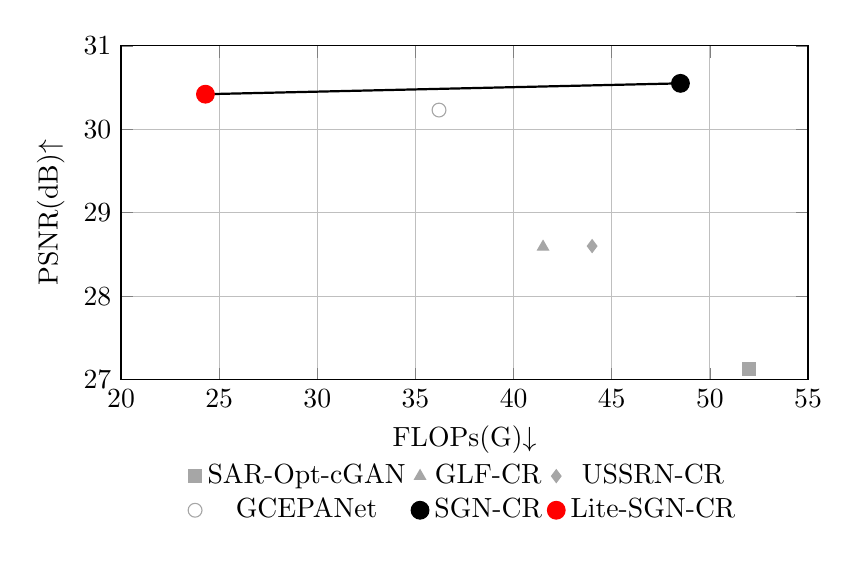
\begin{tikzpicture}
	\begin{axis}[
		width=0.85\textwidth,
		height=0.48\textwidth,
		xlabel={FLOPs(G)$\downarrow$},
		ylabel={PSNR(dB)$\uparrow$},
		grid=both,
		xmin=20, xmax=55,
		ymin=27.0, ymax=31.0,
		legend style={
			at={(0.5,-0.22)},
			anchor=north,
			legend columns=3,
			draw=none,
			fill=none
		},
	]

	% Baselines (gray, different markers)
	\addplot[only marks, mark=square*, mark size=2.3pt, gray!70] coordinates {(52.0,27.13)};
	\addlegendentry{SAR-Opt-cGAN}

	\addplot[only marks, mark=triangle*, mark size=2.3pt, gray!70] coordinates {(41.5,28.59)};
	\addlegendentry{GLF-CR}

	\addplot[only marks, mark=diamond*, mark size=2.3pt, gray!70] coordinates {(44.0,28.60)};
	\addlegendentry{USSRN-CR}

	\addplot[only marks, mark=o, mark size=2.5pt, gray!70] coordinates {(36.2,30.23)};
	\addlegendentry{GCEPANet}

	% SGN-CR (black)
	\addplot[only marks, mark=*, mark size=3.2pt, black] coordinates {(48.5,30.55)};
	\addlegendentry{SGN-CR}

	% Lite-SGN-CR (red)
	\addplot[only marks, mark=*, mark size=3.2pt, red] coordinates {(24.3,30.42)};
	\addlegendentry{Lite-SGN-CR}

	% Arrow only
	\draw[->, thick]
		(axis cs:48.5,30.55) -- (axis cs:24.3,30.42);

	\end{axis}
	\end{tikzpicture}
\end{figure}

从整体分布趋势来看,Lite-SGN-CR 更接近低复杂度与较高性能兼顾的区域,体现出较好的性能与效率权衡关系。

综合来看,Lite-SGN-CR 在保持重建性能基本稳定的前提下,实现了显著的模型压缩与计算效率提升。该结果表明,通过针对性结构重构与算子级优化,可以在当前网络框架下实现有效压缩,为资源受限场景下的实际部署提供支持。

\subsection{消融实验分析}

为深入分析 Lite-SGN-CR 各项轻量化策略的合理性与必要性,本文围绕网络结构重构过程中涉及的关键改动开展系统消融实验。实验主要从以下四个方面进行分析:光学分支通道压缩比例、SAR 分支结构轻量化、跨模态融合模块轻量化以及累积式轻量化路径。通过逐项替换与对比,可以揭示 Lite-SGN-CR 在保持性能稳定的同时实现复杂度压缩的内在机制。

\subsubsection{光学分支通道配置消融}

为进一步分析光学分支网络容量对重建性能与计算复杂度的影响,本文对光学编码器各阶段通道数进行一致缩放,构建不同宽度配置进行对比实验。具体而言,基准配置采用四阶段通道数 ${32, 64, 128, 256}$,并分别设置 0.75×、0.5× 与 0.25× 的宽度缩放版本,对应表中的 C1、C2、C3 与 C4。

在该实验中,SAR 编码分支与跨模态融合模块均保持为 Lite-SGN-CR 的默认结构,仅对光学编码器通道规模进行一致缩放,以确保实验的单变量可比性。

从表 \ref{tab:Lite-channel-config-ablation} 可以观察到,随着通道数逐渐缩减,模型参数规模与 FLOPs 近似线性下降,说明网络宽度对整体计算开销具有显著影响。相较于 C1,C3 在参数量与 FLOPs 分别下降约 34\% 与 36\% 的同时,PSNR 仅下降 0.08 dB,SSIM 变化幅度小于 0.001,表明模型在该容量范围内处于性能平台区间,网络表达能力尚未成为主要瓶颈。

然而,当通道配置进一步压缩至 C4 时,PSNR 与 SSIM 指标出现明显下降,说明光学分支容量已不足以支撑复杂光谱重建任务,尤其在厚云区域结构恢复与细节保持方面表现出不稳定现象。

\begin{table}[!htbp]
\renewcommand{\arraystretch}{1.5}
\centering
\bicaption[\xiaosi 光学分支通道配置消融实验]
{\wuhao 光学分支通道配置消融实验}
{\wuhao Ablation study on optical branch width configuration}
\label{tab:Lite-channel-config-ablation}
\wuhao
\begin{tabular}{@{}>{\songti\wuhao}p{0.24\textwidth}>{\centering\arraybackslash\songti\wuhao}p{0.14\textwidth}>{\centering\arraybackslash\songti\wuhao}p{0.14\textwidth}>{\centering\arraybackslash\songti\wuhao}p{0.14\textwidth}>{\centering\arraybackslash\songti\wuhao}p{0.14\textwidth}@{}}
\toprule[1.5pt]
通道配置 & Params(M) & FLOPs(G) & PSNR(dB)$\uparrow$ & SSIM$\uparrow$ \\
\hline
C1: [32,64,128,256] & 7.90 & 36.0 & 30.58 & 0.8994 \\
C2: [24,48,96,192] & 6.60 & 30.0 & 30.55 & 0.8990 \\
\textbf{C3: [16,32,64,128]} & \textbf{5.20} & \textbf{23.0} & \textbf{30.50} & \textbf{0.8984} \\
C4: [8,16,32,64] & 4.10 & 16.0 & 30.20 & 0.8935 \\
\bottomrule[1.5pt]
\end{tabular}
\end{table}

该结果进一步验证了 Lite-SGN-CR 采用“模态不对称容量分配”策略的合理性。即在保证光学分支具备基本光谱重建能力的前提下,将冗余通道规模压缩至性能平台区间内的最小可行容量,从而在不显著损失重建质量的前提下实现计算复杂度的有效降低。基于上述分析,本文最终选取 C3 配置(${16, 32, 64, 128}$)作为 Lite-SGN-CR 的默认宽度配置。

\subsubsection{SAR 编码分支轻量化结构消融}

原始 SGN-CR 中,SAR 分支包含三个尺度特征层级,通道数分别为 64、128、256,每一尺度均堆叠 3 个 ResNet 风格的 SAR-block。该结构能够获得较大的感受野,但存在层级堆叠冗余与计算开销偏高的问题。

在 Lite-SGN-CR 中,SAR 分支被重构为一个初始特征嵌入层与两个逐级下采样编码层组成的浅层结构。具体而言,输入 SAR 图像首先通过一个 $3\times3$、stride=2 的卷积生成 32 通道特征图,随后仅使用两个 Lite-SAR-block 分别生成 64 通道与 128 通道的多尺度结构表示。Lite-SAR-block 采用 DWConv 替代原有 ResNet 风格卷积模块,同时将每一尺度的 block 堆叠数由 3 降为 1,层级数由 3 层压缩为 2 层。

为进一步验证 SAR 分支的容量下界,本文在 Lite 结构基础上构建过度压缩版本的 SAR Encoder,将各阶段通道规模进一步减半,即采用 16 → 32 → 64 的两层级 DWConv 结构。在该实验中,光学分支通道配置固定为 C3,跨模态融合模块保持为 Lite-CMCA,推理阶段数保持一致,仅替换 SAR 编码结构以保证单变量对比公平性。

从表 \ref{tab:Lite-SAR-ablation} 可以观察到,相较于原始残差结构,Lite SAR 编码器在参数量与 FLOPs 分别下降约 18\% 与 19\% 的同时,PSNR 与 SSIM 仅产生轻微波动,说明 SAR 分支存在一定的可压缩空间。在保证结构先验提取能力的前提下,浅层 DWConv 结构已能够有效建模地物轮廓与空间连续性。

\begin{table}[!htbp]
	\renewcommand{\arraystretch}{1.5}
	\centering
	\bicaption[\xiaosi SAR 分支结构消融实验]
	{\wuhao SAR 分支结构消融实验}
	{\wuhao Ablation study on SAR encoder structure}
	\label{tab:Lite-SAR-ablation}
	\wuhao
	\begin{tabular}{@{}>{\arraybackslash\songti\wuhao}p{0.24\textwidth}>{\centering\arraybackslash\songti\wuhao}p{0.14\textwidth}>{\centering\arraybackslash\songti\wuhao}p{0.14\textwidth}>{\centering\arraybackslash\songti\wuhao}p{0.14\textwidth}>{\centering\arraybackslash\songti\wuhao}p{0.14\textwidth}@{}}
		\toprule[1.5pt]
		模型变体 & Params(M) & FLOPs(G) & PSNR(dB)$\uparrow$ & SSIM$\uparrow$ \\
		\hline
		\makecell[l]{原始 SAR 编码器 \\ (64-128-256)} & 6.40 & 28.5 & 30.56 & 0.8992 \\
		\textbf{\makecell[l]{Lite SAR 编码器 \\ (32-64-128)}} & \textbf{5.20} & \textbf{23.0} & \textbf{30.52} & \textbf{0.8986} \\
		\makecell[l]{过度压缩 SAR 编码器 \\ (16-32-64)} & 4.85 & 21.0 & 30.20 & 0.8940 \\
		\bottomrule[1.5pt]
	\end{tabular}
\end{table}

然而,当通道规模进一步减半至 16-32-64 时,重建性能出现明显下降,尤其在厚云区域结构恢复方面表现出边缘细节减弱与局部纹理不稳定现象。这表明虽然 SAR 分支主要承担结构骨架提取功能,但仍需保持基本的多尺度表达能力以支撑跨模态融合过程。

上述结果表明,网络宽度与重建性能之间并非线性关系,而是存在明显的性能平台区间与容量临界点。在容量处于平台区间内时,适度压缩通道规模不会显著影响模型的表达能力;然而当容量低于临界阈值后,光学分支的特征建模能力将成为性能瓶颈,从而导致重建质量明显下降。

综合复杂度压缩比例与性能变化趋势,C3 配置位于性能平台区间的下界附近,在保证重建质量基本稳定的前提下实现了较大幅度的计算开销下降。

\subsubsection{跨模态融合模块轻量化消融}

为降低跨模态特征交互过程中的计算开销,Lite-SGN-CR 对原始 CMCA 模块进行了结构级简化。原 CMCA 模块在深层语义阶段采用标准卷积与通道投影操作进行跨模态特征交互,而 Lite-CMCA 在保持交叉注意力机制框架不变的前提下,将部分 $3\times3$ 标准卷积替换为 DWConv,并减少冗余通道变换操作,从而实现计算复杂度的有效压缩。

为验证该轻量化改动的有效性,本文设置三组对比实验:完全移除跨模态融合机制、采用原始 CMCA 模块,以及采用 Lite-CMCA 模块。在该实验中,SAR 编码分支固定为 Lite 结构,光学分支通道配置固定为 C3,推理阶段数保持一致,仅对融合模块进行替换,以保证单变量对比的公平性。

\begin{table}[!htbp]
	\renewcommand{\arraystretch}{1.5}
	\centering
	\bicaption[\xiaosi 跨模态融合模块消融实验]
	{\wuhao 跨模态融合模块消融实验}
	{\wuhao Ablation study on cross-modal fusion module}
	\label{tab:Lite-fusion-ablation}
	\wuhao
	\begin{tabular}{@{}>{\raggedright\arraybackslash\songti\wuhao}p{0.24\textwidth}
	>{\centering\arraybackslash\songti\wuhao}p{0.14\textwidth}
	>{\centering\arraybackslash\songti\wuhao}p{0.14\textwidth}
	>{\centering\arraybackslash\songti\wuhao}p{0.14\textwidth}
	>{\centering\arraybackslash\songti\wuhao}p{0.14\textwidth}@{}}
		\toprule[1.5pt]
		融合策略 & Params(M) & FLOPs(G) & PSNR(dB)$\uparrow$ & SSIM$\uparrow$ \\
		\hline
		无融合模块 & 4.90 & 21.5 & 30.10 & 0.8905 \\
		原始 CMCA 模块 & 5.40 & 24.5 & 30.54 & 0.8989 \\
		\textbf{Lite-CMCA 模块} & \textbf{5.20} & \textbf{23.0} & \textbf{30.50} & \textbf{0.8984} \\
		\bottomrule[1.5pt]
	\end{tabular}
\end{table}

从表 \ref{tab:Lite-fusion-ablation} 可以观察到,在完全移除跨模态融合机制后,PSNR 与 SSIM 分别下降约 0.4 dB 与 0.008,表明跨模态结构引导在云去除任务中发挥关键作用。该机制能够利用 SAR 所提供的稳定几何结构信息,对光学特征进行结构一致性约束与特征层面对齐,从而有效缓解厚云区域的纹理伪生成与结构失真问题。

在保留融合机制的前提下,Lite-CMCA 相较于原始 CMCA 在参数量与 FLOPs 分别下降约 3.7\% 与 6.1\% 的同时,PSNR 仅下降 0.04 dB,SSIM 基本保持稳定。该结果表明,通过对融合模块内部结构进行重构与算子级优化,可以在显著降低计算开销的同时维持重建性能。

上述分析说明,跨模态融合机制是提升云去除性能的核心组成部分,而其内部实现方式仍存在复杂度压缩空间。通过引入轻量卷积结构并简化通道变换路径,Lite-CMCA 在保持结构引导能力的前提下有效降低了计算负担,实现了功能表达与计算复杂度之间的平衡。

\subsubsection{累积式轻量化路径}

为进一步验证 Lite-SGN-CR 各项轻量化改动的累积贡献,并分析性能与复杂度之间的整体权衡关系,本文设计分阶段累积式轻量化路径。以原始 SGN-CR 为起点,在保持训练策略、输入分辨率与评价指标一致的前提下,分析各阶段结构改动对模型复杂度与重建性能的影响趋势。除原始 SGN-CR 外,其余 Lite 系列路径变体均在递归阶段数固定为 3 的条件下进行训练与测试,以保证比较结果的一致性。

如表 \ref{tab:cumulative_lite_path} 所示,随着轻量化改动的逐步引入,模型复杂度呈现出单调下降趋势,而重建性能整体保持稳定,体现出明显的累积压缩效应。首先,在引入 Lite-SAR 后,参数规模与 FLOPs 均显著降低,而 PSNR 与 SSIM 仅出现极小幅波动,说明 SAR 分支存在较大的结构冗余与可压缩空间。随后,对光学分支实施通道规模缩放后,模型复杂度进一步下降,在 C3 配置之前性能仍处于平台区间,表明在该容量范围内光学分支的光谱建模能力尚未成为性能瓶颈。

\begin{table}[!htbp]
\renewcommand{\arraystretch}{1.5}
\centering
\bicaption[\xiaosi 累积式轻量化路径对比实验]
{\wuhao 累积式轻量化路径对比实验}
{\wuhao Cumulative ablation on progressive lightweighting path}
\label{tab:cumulative_lite_path}
\wuhao
\begin{tabular}{@{}>{\raggedright\arraybackslash\songti\wuhao}p{0.32\textwidth}
>{\centering\arraybackslash\songti\wuhao}p{0.12\textwidth}
>{\centering\arraybackslash\songti\wuhao}p{0.12\textwidth}
>{\centering\arraybackslash\songti\wuhao}p{0.12\textwidth}
>{\centering\arraybackslash\songti\wuhao}p{0.12\textwidth}@{}}
\toprule[1.5pt]
路径变体 & Params(M)$\downarrow$ & FLOPs(G)$\downarrow$ & PSNR(dB)$\uparrow$ & SSIM$\uparrow$ \\
\hline
P0: SGN-CR & 10.80 & 48.5 & 30.58 & 0.8994 \\
P1: P0 + Lite-SAR & 9.60 & 44.0 & 30.57 & 0.8992 \\
P2: P1 + Optical Width@C2 & 8.20 & 36.0 & 30.56 & 0.8990 \\
P3: P1 + Optical Width@C3 & 6.80 & 28.0 & 30.52 & 0.8986 \\
P4: P3 + Lite-CMCA & 6.60 & 27.0 & 30.50 & 0.8984 \\

\textbf{P5: Lite-SGN-CR} & \textbf{5.20} & \textbf{23.0} & \textbf{30.50} & \textbf{0.8984} \\
\bottomrule[1.5pt]
\end{tabular}
\end{table}

在此基础上,将原始 CMCA 替换为 Lite-CMCA 后,模型在保持跨模态结构引导路径完整性的前提下进一步降低计算开销,且性能变化幅度有限,表明融合模块的功能贡献主要来源于跨模态信息交互机制,而非其高复杂度实现形式。

综合上述阶段性压缩结果可以看出,Lite-SGN-CR 的轻量化过程并非对网络进行均匀削减,而是针对不同模态分支与关键融合模块实施有选择性的复杂度优化,从而在保持重建质量基本稳定的前提下,实现模型规模与推理成本的协同下降。

\subsection{渐进式去云策略性能分析}

为分析渐进式递归细化机制在 Lite-SGN-CR 中的性能收益,本节从迭代阶段数选择与门控机制有效性两个方面进行实验验证。实验仅改变递归阶段数。所有测试均在输入分辨率为 $256\times256$、batch size=1 条件下统计。

\subsubsection{不同渐进阶段数下的性能变化}

在 Lite-SGN-CR 基础上,设置不同递归迭代次数 $T \in \{1,2,3,4,5\}$ 进行对比实验。其中,$T=1$ 表示单次推理结果,$T>1$ 表示在初始估计基础上进行多轮共享参数的递归更新。表~\ref{tab:progressive_stage} 给出了不同迭代次数下的性能与计算开销对比结果。

从结果可以观察到,当 $T$ 从 1 增加至 2 时,PSNR 提升约 0.58 dB,表明首次递归细化能够显著修正单次预测中的残余误差。随着迭代次数进一步增加,性能继续提升但增幅逐渐减缓,表现出明显的收益递减趋势。当 $T \ge 4$ 时,各项指标基本趋于饱和,部分指标出现轻微波动,说明过多迭代可能在局部区域引入额外扰动而难以带来稳定增益。这一现象可能源于递归更新过程中误差的逐步传播与累积。当模型在已接近收敛状态下继续进行全局修正时,局部区域的微小偏差可能被反复放大,从而导致整体指标难以进一步提升甚至出现轻微回落。

\begin{table}[!htbp]
	\renewcommand{\arraystretch}{1.5}
	\centering
	\bicaption[\xiaosi 不同渐进阶段数下的性能与计算开销对比]
	{\wuhao 不同渐进阶段数下的性能与计算开销对比}
	{\wuhao Performance and computational cost under different progressive stages}
	\label{tab:progressive_stage}
	\wuhao
	\begin{tabular}{@{}>{\centering\arraybackslash\songti\wuhao}p{0.14\textwidth}>{\centering\arraybackslash\songti\wuhao}p{0.13\textwidth}>{\centering\arraybackslash\songti\wuhao}p{0.12\textwidth}>{\centering\arraybackslash\songti\wuhao}p{0.12\textwidth}>{\centering\arraybackslash\songti\wuhao}p{0.12\textwidth}>{\centering\arraybackslash\songti\wuhao}p{0.13\textwidth}@{}}
		\toprule[1.5pt]
		渐进阶段数 & Params(M) & FLOPs(G) & Latency(ms)$\downarrow$ & PSNR(dB)$\uparrow$ & SSIM$\uparrow$ \\
		\hline
		1 & 5.20 & 18.6 & 42.3 & 29.84 & 0.8912 \\
		2 & 5.20 & 37.2 & 84.5 & 30.42 & 0.8968 \\
		3 & 5.20 & 55.8 & 126.9 & 30.68 & 0.8991 \\
		4 & 5.20 & 74.4 & 169.4 & 30.75 & 0.8998 \\
		5 & 5.20 & 92.0 & 239.1 & 30.34 & 0.8998 \\
		\bottomrule[1.5pt]
	\end{tabular}
\end{table}

与此同时,推理阶段的 FLOPs 与延迟时间随 $T$ 近似线性增长。当阶段数由 1 增加至 5 时,计算量与推理时间约提升至原来的 5 倍,说明渐进式性能提升是以线性计算代价为前提实现的。

从图~\ref{fig:stage_performance-cost}(a) 可以看出,随着渐进阶段数由 1 增加至 4,PSNR 与 SSIM 指标均呈现稳定上升趋势。其中,PSNR 从 29.84~dB 提升至 30.75~dB,SSIM 从 0.8912 提升至 0.8998,表明多阶段递归细化能够逐步修正残余云区误差,并增强重建结果的结构一致性与纹理细节表达能力。

从机理上分析,渐进式策略通过参数共享的多阶段重建方式,使网络在每一阶段对前一阶段输出进行残差补偿与细节优化。初始阶段主要恢复整体结构信息,而后续阶段则进一步细化高频纹理与光谱特征,因此性能随阶段数增加而持续提升。然而,当阶段数增加至 5 时,PSNR 出现下降趋势,而 SSIM 基本保持稳定,说明过多的递归迭代可能引入误差累积或过度平滑现象,从而削弱重建质量。

综合来看,4 阶段在性能提升与稳定性之间取得了较优平衡。

图~\ref{fig:stage_performance-cost}(b) 展示了不同渐进阶段数下计算复杂度的变化情况。可以观察到,FLOPs 与 Latency 均随阶段数呈近似线性增长趋势。这是由于各阶段共享同一组网络参数,但前向传播次数随阶段数增加而等比例叠加,因此总体计算量呈线性放大。

\begin{figure}[!htbp]
\centering
\bicaption[\xiaosi 不同渐进阶段数下的性能与计算复杂度变化趋势]
{\wuhao 不同渐进阶段数下的性能与计算复杂度变化趋势}
{\wuhao Performance and computational cost under different progressive stages}
\label{fig:stage_performance-cost}
% 微调参数(只改这里即可)
\def\StageGroupShift{-18mm}   % 整组左右平移
\def\StageLegendY{-7.5mm}     % 图例相对主图底部的垂直位置
\def\StageSubcapY{-18.0mm}    % (a)/(b) 相对主图底部的垂直位置
\def\StageBBoxY{-22.0mm}      % 包围盒向下延伸,避免裁切
\def\StageLegendXLeft{0pt}    % 左图图例水平微调
\def\StageLegendXRight{0pt}   % 右图图例水平微调
\def\StageSubcapXLeft{0pt}    % 左图(a)水平微调
\def\StageSubcapXRight{0pt}   % 右图(b)水平微调
\makebox[\textwidth][c]{\hspace*{\StageGroupShift}%
% ---------- (a) 性能 ----------
\begin{minipage}[t]{0.40\textwidth}
\centering
\begin{tikzpicture}

% ---------------- 左轴:PSNR ----------------
\begin{axis}[
    name=perfbox,
    scale only axis,
    trim axis left,
    trim axis right,
    width=0.95\linewidth,
    height=6.2cm,
    ylabel=\empty, % 取消外部 ylabel
    xmin=1, xmax=5,
    xtick={1,2,3,4,5},
    ymin=29.75, ymax=30.85,
    grid=both,
    grid style={line width=.2pt, draw=gray!30},
]
\addplot[black, thick, mark=*] coordinates {
  (1,29.84) (2,30.42) (3,30.68) (4,30.75) (5,30.34)
};

% 图内标注:PSNR
\node[anchor=north west] at (rel axis cs:0.02,0.98) {\small PSNR (dB)};
\end{axis}

% ---------------- 右轴:SSIM ----------------
\begin{axis}[
    scale only axis,
    trim axis left,
    trim axis right,
    width=0.95\linewidth,
    height=6.2cm,
    xmin=1, xmax=5,
    xtick=\empty,
    axis x line=none,
    axis y line*=right,
    ylabel=\empty, % 取消外部 ylabel
    ymin=0.890, ymax=0.900,
    ytick={0.890,0.892,0.894,0.896,0.898,0.900},
    yticklabel style={
        xshift=-2pt,
        /pgf/number format/fixed,
        /pgf/number format/precision=3
    },
]
\addplot[black, thick, dashed, mark=square*] coordinates {
  (1,0.8912) (2,0.8968) (3,0.8991) (4,0.8998) (5,0.8998)
};

% 图内标注:SSIM(右上角)
\node[anchor=north east] at (rel axis cs:0.98,0.98) {\small SSIM};

% 右下角 x 轴标题
\node[anchor=south east] at (axis cs:5,0.890) {\small 渐进阶段数};
\end{axis}

% legend(保持你原样式)
\node[draw, fill=white, inner sep=4pt, anchor=north]
at ([xshift=\StageLegendXLeft,yshift=\StageLegendY]perfbox.south) {%
  \begin{tikzpicture}[baseline=-0.6ex]
    % PSNR: 实线+圆点
    \draw[black, thick] (0,0) -- (0.9,0);
    \draw plot[mark=*, mark size=2.6pt] coordinates {(0.5,0)};
    \node[anchor=west] at (1.05,0) {PSNR};

    % SSIM: 虚线+方块(用 marker,更像曲线上方块)
    \draw[black, thick, dashed] (2.5,0) -- (3.15,0);
    \draw plot[mark=square*, mark size=2.8pt] coordinates {(2.80,0)};
    \node[anchor=west] at (3.25,0) {SSIM};
  \end{tikzpicture}%
};
\node[anchor=north]
at ([xshift=\StageSubcapXLeft,yshift=\StageSubcapY]perfbox.south)
{\wuhao (a) 性能变化趋势};
% 强制统一包围盒,避免右轴刻度长度影响整体居中
\path[use as bounding box] ([yshift=\StageBBoxY]perfbox.south west) rectangle (perfbox.north east);

\end{tikzpicture}
\end{minipage}%
\hspace{0.12\textwidth}
% ---------- (b) 复杂度 ----------
\begin{minipage}[t]{0.40\textwidth}
\centering
\begin{tikzpicture}

% ---------------- 左轴:FLOPs ----------------
\begin{axis}[
      name=costbox,
      scale only axis,
      trim axis left,
      trim axis right,
      width=0.95\linewidth,
      height=6.2cm,
      ylabel=\empty, % 取消外部 ylabel
      xmin=1, xmax=5,
      xtick={1,2,3,4,5},
      ymin=0, ymax=100,
      ytick={0,20,40,60,80,100},
      grid=both,
      grid style={line width=.2pt, draw=gray!30},
]
\addplot[black, thick, mark=*] coordinates {
  (1,18.6) (2,37.2) (3,55.8) (4,74.4) (5,92.0)
};

% 图内标注:FLOPs
\node[anchor=north west] at (rel axis cs:0.02,0.98) {\small FLOPs (G)};
\end{axis}

% ---------------- 右轴:Latency ----------------
\begin{axis}[
      scale only axis,
      trim axis left,
      trim axis right,
      width=0.95\linewidth,
      height=6.2cm,
      xmin=1, xmax=5,
      xtick=\empty,
      axis x line=none,
      axis y line*=right,
      ylabel=\empty, % 取消外部 ylabel
      ymin=0, ymax=260,
      ytick={0,50,100,150,200,250},
      yticklabel style={xshift=-2pt},
]
\addplot[black, thick, dashed, mark=square*] coordinates {
  (1,42.3) (2,84.5) (3,126.9) (4,169.4) (5,239.1)
};

% 图内标注:Latency(右上角)
\node[anchor=north east] at (rel axis cs:0.98,0.98) {\small Latency (ms)};

% 右下角 x 轴标题
\node[anchor=south east] at (axis cs:5,0) {\small 渐进阶段数};
\end{axis}

% legend(与左图一致)
\node[draw, fill=white, inner sep=4pt, anchor=north]
at ([xshift=\StageLegendXRight,yshift=\StageLegendY]costbox.south) {%
  \begin{tikzpicture}[baseline=-0.6ex]
    % FLOPs: 实线+圆点
    \draw[black, thick] (0,0) -- (0.9,0);
    \draw plot[mark=*, mark size=2.6pt] coordinates {(0.5,0)};
    \node[anchor=west] at (1.05,0) {FLOPs};

    % Latency: 虚线+方块
    \draw[black, thick, dashed] (2.60,0) -- (3.50,0);
    \draw plot[mark=square*, mark size=2.8pt] coordinates {(3.0,0)};
    \node[anchor=west] at (3.40,0) {Latency};
  \end{tikzpicture}%
};
\node[anchor=north]
at ([xshift=\StageSubcapXRight,yshift=\StageSubcapY]costbox.south)
{\wuhao (b) 计算复杂度变化趋势};
% 强制统一包围盒,避免右轴刻度长度影响整体居中
\path[use as bounding box] ([yshift=\StageBBoxY]costbox.south west) rectangle (costbox.north east);

\end{tikzpicture}
\end{minipage}
}
\end{figure}

具体而言,当阶段数由 1 增至 5 时,FLOPs 从 18.6~G 增至 92.0~G,Latency 从 42.3~ms 增至 239.1~ms,增长幅度显著。该结果验证了渐进式策略在不增加模型参数规模的前提下,通过增加推理轮次换取性能提升的特性。

因此,渐进阶段数的选择本质上体现为重建性能与计算代价之间的权衡问题。

\begin{figure}[!htbp]
  \centering
  \bicaption[\xiaosi 渐进阶段数的性能—复杂度权衡关系]
  {\wuhao 渐进阶段数的性能—复杂度权衡关系}
  {\wuhao Performance-complexity trade-off of progressive stages}
  \label{fig:stage_tradeoff}

  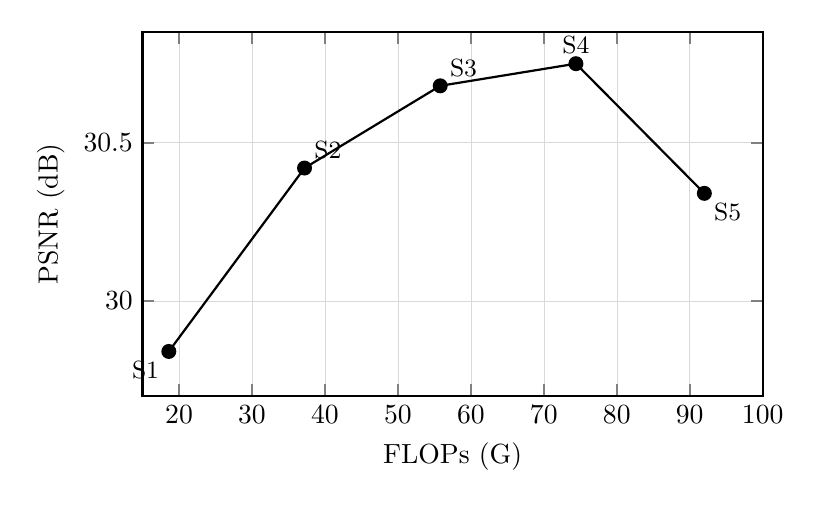
\begin{tikzpicture}
    \begin{axis}[
      width=0.78\textwidth,
      height=6.2cm,
      xlabel={FLOPs (G)},
      ylabel={PSNR (dB)},
      xmin=15, xmax=100,
      ymin=29.7, ymax=30.85,
      grid=both,
      grid style={line width=.2pt, draw=gray!30},
      axis line style={line width=0.8pt},
      tick style={line width=0.8pt},
      clip=false, % allow labels slightly outside plot without clipping
    ]

      \addplot[black, thick, solid, mark=*, mark size=2.3pt] coordinates {
        (18.6,29.84)
        (37.2,30.42)
        (55.8,30.68)
        (74.4,30.75)
        (92.0,30.34)
      };

      % Labels with offsets (no overlap with points/line)
      \node[anchor=north east] at (axis cs:18.6,29.84) {\small S1};
      \node[anchor=south west] at (axis cs:37.2,30.42) {\small S2};
      \node[anchor=south west] at (axis cs:55.8,30.68) {\small S3};
      \node[anchor=south]      at (axis cs:74.4,30.75) {\small S4};
      \node[anchor=north west] at (axis cs:92.0,30.34) {\small S5};

    \end{axis}
  \end{tikzpicture}
\end{figure}

为进一步分析渐进阶段数对模型效率的综合影响,图~\ref{fig:stage_tradeoff} 给出了不同阶段数在性能与计算复杂度平面上的分布关系。从图中可以看出,当阶段数由 1 增至 4 时,PSNR 随 FLOPs 的增加而明显提升,表明额外计算开销能够有效转化为性能收益;而当阶段数进一步增加至 5 时,尽管计算复杂度持续上升,但性能反而出现下降,呈现明显的收益递减现象。

从性能–复杂度分布位置来看,第 4 阶段位于性能最高且计算代价相对可控的区域,是当前结构与训练策略下的最优递归深度选择。相比之下,第 5 阶段在计算效率上并不具备优势。

上述结果表明,在轻量化模型框架下,合理设置渐进阶段数能够有效弥补模型容量受限所带来的性能损失,但过度递归将削弱整体效率优势。因此,本研究选择 $T=3$ 作为默认推理设置。在该配置下,模型在保持可控计算复杂度的同时获得较为稳定且显著的性能提升。

\subsubsection{门控机制有效性验证}

为验证门控残差机制在递归细化过程中的稳定性与有效性,在固定迭代次数 $T=3$ 条件下,对比以下两种更新形式:

无门控递归(no-gate):
\begin{equation}
x_{t+1} = x_t + \Delta x_t
\end{equation}

门控残差递归(gated):
\begin{equation}
x_{t+1} = x_t + M_t \odot \Delta x_t
\end{equation}

其中,$\Delta x_t$ 表示当前轮预测与估计之间的残差更新项,$M_t$ 为逐像素门控权重。表~\ref{tab:gate_ablation} 给出了两种递归形式的性能对比结果。

\begin{table}[!htbp]
	\renewcommand{\arraystretch}{1.5}
	\centering
	\bicaption[\xiaosi 门控机制有效性对比($T=3$)]
	{\wuhao 门控机制有效性对比($T=3$)}
	{\wuhao Comparison of gating mechanism effectiveness ($T=3$)}
	\label{tab:gate_ablation}
	\wuhao
	\begin{tabular}{@{}>{\arraybackslash\songti\wuhao}p{0.18\textwidth}>{\centering\arraybackslash\songti\wuhao}p{0.16\textwidth}>{\centering\arraybackslash\songti\wuhao}p{0.16\textwidth}>{\centering\arraybackslash\songti\wuhao}p{0.16\textwidth}@{}}
		\toprule[1.5pt]
		渐进式方法 & PSNR(dB)$\uparrow$ & SSIM$\uparrow$ & MAE$\downarrow$ \\
		\hline
		no-gate & 30.54 & 0.8976 & 0.0243 \\
		gated  & 30.68 & 0.8991 & 0.0238 \\
		\bottomrule[1.5pt]
	\end{tabular}
\end{table}

可以观察到,在相同迭代次数条件下,引入门控机制后 PSNR 提升约 0.14 dB,SSIM 同步提升,MAE 略有下降。无门控递归在多轮更新过程中对全图区域进行均匀修正,易在已恢复区域引入累积扰动;而门控残差机制通过逐像素调节更新强度,使修正更加集中于高不确定区域,从而提升了递归细化的稳定性与最终重建质量。

上述结果表明,在不增加模型参数规模的前提下,门控机制能够有效增强渐进式推理的稳定性,并进一步释放递归细化带来的性能潜力。

\section{本章小结}

本章围绕 Lite-SGN-CR 轻量化网络的结构设计与性能表现展开系统分析。在保持第三章提出的跨模态引导框架不变的前提下,通过引入深度可分离卷积、通道压缩与轻量化融合模块,对模型进行针对性结构优化。综合对比实验结果表明,Lite-SGN-CR 在 PSNR、SSIM、SAM 与 MAE 等重建指标上与原始 SGN-CR 保持接近水平,说明轻量化设计在有效压缩模型规模的同时,未显著削弱关键结构表达能力。

复杂度与推理效率分析进一步验证,Lite-SGN-CR 在参数规模、FLOPs 及推理延迟方面均实现显著下降,体现出明显的计算效率优势。消融实验结果显示,SAR 分支轻量化、光学分支通道压缩以及跨模态融合模块简化等设计在降低冗余计算路径的同时,仍然保留了必要的结构与语义信息建模能力,验证了各模块改进的合理性。

在此基础上,本章进一步引入渐进式递归细化机制,通过共享参数的多轮推理实现对单次预测结果的持续修正。实验结果表明,在适当迭代次数下,该机制能够在不增加模型参数规模的前提下进一步提升重建稳定性,并提供可调节的精度–效率权衡能力。

综上所述,Lite-SGN-CR 在保证重建质量基本稳定的同时,实现了显著的模型压缩与推理效率提升,并通过渐进式细化策略增强了轻量化模型的性能补偿能力,为资源受限环境下的遥感图像云去除任务提供了一种兼顾精度与效率的实用化解决方案。
